\documentclass{UCreport} 



\usepackage[authoryear,comma,round]{natbib}
\usepackage{hyperref,graphicx}
\usepackage[separate-uncertainty=true,multi-part-units=single]{siunitx}

\usepackage{caption}
\usepackage[list=true,listformat=simple]{subcaption}
\makeatletter
\g@addto@macro\p@subfigure{.}
\makeatother

% \usepackage[margin=1.5cm, left=3cm ,twoside]{geometry}

\usepackage[para]{footmisc}

\usepackage[super]{nth}

\usepackage{amsmath,amssymb}

\DeclareSIUnit{\arcsec}{''}
\DeclareSIUnit{\au}{\mathrm{AU}}
\DeclareSIUnit{\mag}{\mathrm{mag}}
\DeclareSIUnit{\px}{\mathrm{px}}

\usepackage[utf8]{inputenc}
\usepackage[T1]{fontenc}
\usepackage{newunicodechar}

\DeclareRobustCommand{\okina}{%
  \raisebox{\dimexpr\fontcharht\font`A-\height}{%
    \scalebox{0.8}{`}%
  }%
}
\newunicodechar{ʻ}{\okina}
\newcommand{\omuamua}{\okina Oumuamua }


% \title{ASTR480 Final Report:\\
% \textit{Asteroids in TESS}
% }
% \author{Brayden Leicester \\ 
% \textit{61352063} \\
% [1ex]\small{Supervisors: Michele Bannister and Ryan Ridden-Harper}
% }
\begin{document}



%----------- Report information ---------

\logo{logos/UC.png}
\school{\textbf{School of Physical and Chemical Sciences}}
\course{\textbf{ASTR480}}
\student{\textbf{Brayden Leicester}}
\supervisor{Dr Michele Bannister and Dr Ryan Ridden-Harper}
\ttitle{Asteroids in TESS} %title of the file


%----------- Init -------------------

\buildmargins % display margins
\buildcover % create the front cover of the document



%------------ Declaration ----------------
\pagenumbering{roman}
\addcontentsline{toc}{section}{Declaration}
\declaration

I certify that content of this report was mostly my own work.
\\

My supervisors helped by proofreading the report and offering feedback. As well as providing useful insight into problems when I was stuck.\\

Graduate students, X and Y, helped me understand ... \\

The derivation in section 3 was taken from ... \\

\autoref{Fig:FreqVsDiam} has been constructed from data from the Light Curve Database (LCDB) \citet{Warner2009}, as cited in text. That data has being built suplimented with my own work in the corrseponding Figure %TODO

\vspace{2cm}
\begin{centering}
  \textbf{\student}\par
\end{centering}

\newpage

%------------ Abstract ----------------

\addcontentsline{toc}{section}{Abstract}
\abstract

This is where the abstract goes. \\

This is the next paragraph.

% %*Background

% %*Methods

% %*Main Results

% %*Conclusion

\newpage
%------------ Contents pages ----------------

\toc % creates the table of contents

\addcontentsline{toc}{section}{List of Figures}
\listoffigures
\newpage
\addcontentsline{toc}{section}{List of Tables}
\listoftables
\newpage

%------------ Report body ----------------
\pagenumbering{arabic}

\section{Introduction}\label{Sec:Intro}

%To get all asteroids in TESS. 
This project aims to find and characterise the light curves of all the asteroids seen by the Transiting Exoplanet Survey Satellite (TESS).
Combining knowledge of these asteroid's positions with the high cadence imaging of TESS should allow for the determination of rotation periods of these small bodies.

\subsection{TESS}\label{SubSec:TESS}

%Why TESS
TESS is a large area, high cadence imaging, space telescope  \citep{Ricker2014}.
TESS is tasked with observing one piece of sky for \qty{27}{\day} at a time (a sector), delivering \qtyproduct{96 x 24}{\degree} full frame images (FFIs) at regular intervals.
These FFIs are built from stacked \qty{2}{\second} exposures, leveraging the short readout times of the 16 CCD cameras on-board.
With the initial cadence for these full frame images set to \qty{30}{\minute}, the time resolution of TESS is unparalleled.
The highest frequency (shortest period) that can be found from time series data like this is at the Nyquist limit, twice the minimum time between images.
Due to the short cadence, the Nyquist frequency of TESS is quite high, \qty{1}{\per\hour}.
This is well sampled enough to characterise most variable stars, as well as find the orbital periods of exoplanets to a high precision.
As the mission was extended, after TESS had already mapped the entire sky, the length of the FFIs has decreased to \qty{10}{\minute} and then later to \qty{200}{\second}.
This decreased in the FFI exposure time comes with a complementary increase in the Nyquist frequency.
This high time resolution and observation area does come at the cost of spatial resolution, as the pixels are each \qty{21}{\arcsec} square.
Of interest here is what such a high sampling rate can do for statistic on the asteroid population.
For bright asteroids the rotation periods should be able to be easily determined from this vast dataset.
The shortest FFIs will be able to accurately determine the rotation periods of all but the fastest rotating asteroids, most of which will be too dim to see in the TESS data.

There have been attempts to find and classify the asteroids in TESS data before.
\citet{Pal2018} proposes that TESS will be a good instrument for solar system object study, and simulate some detections down to \nth{20} visual magnitude, but that good photometry should only be expected to $V \lesssim 19$.
The sentiment of using TESS in this way is shared by \citet{Wong2019}.
The first data release in \citet{Pal2020} catalogues nearly 10,000 asteroid light curves from the first year of TESS operation, and they report that they triple the number of asteroids with accurate rotation periods.
\citet{McNeill2023} also analyse TESS cycle 1, and detect almost 38,000 objects.
They determine reliable rotation periods for about 3,500 asteroids in this sample and show a lack of reliability for objects with periods less than \qty{3}{\hour}.
In the overlap from the data from \citet{Pal2020}, \citeauthor{McNeill2023} find good agreement between the two sets of periods and amplitudes.
The Minor Planet Center (MPC) gets regular updates from TESS thanks to the work of \citet{Woods2021} and their \texttt{LINEAR-TESS} program, which creates tracklets of objects over a day, and then stitches these together to form a track of each asteroid through an FFI.
\citet{Gowanlock2024} uses TESS photometry as well as  observations by the Zwicky Transient Facility \citep[ZTF, ][]{Bellm2018} to get a longer baseline on mutually observed objects while combining ground and space based observations.
There were not very many objects in both samples with known periods for comparison, with only 222 objects analysed, however they demonstrate that the technique is effective.
Fainter and unknown solar system objects can be found by shift and stacking \citep{Holman2019, Payne2019,Rice2020} or taking a fast X-ray transform \citep{Nguyen2024} of the FFI data.

This work aims to extend these studies to more sectors, hence characterising more asteroids.
The aim is to get a volume complete set of asteroid lightcurves and periods, by analysis of the whole sky as seen by TESS using data from more than just the first year of TESS's operation.
I also employ a different data reduction method, reducing the data with the \texttt{TESSreduce} package \citep{Ridden-Harper2021} should increase the accuracy of the photometry due to the improved background subtraction process.
Because of the survey properties, TESS provides a self-consistent way to measure the properties of asteroids over the full sky.
By using the higher cadence FFIs of later TESS sectors, the $P\leq\qty{3}{\hour}$ limit on the accurate periods \citep[as found by ][]{McNeill2023} should be lowered.
Another beneficial part of this work is that as part of a full sky transient survey using TESS, \texttt{TESSELLATE} \citep{TESSELLATE}.
Asteroids can spike the brightness of a pixel for only a few frames while it is passing by.
This can confuse pipelines looking for  transients such as flare stars and supernova, as they can look very similar, having the brightness change in one pixel for a short time.
The goal of finding all the asteroids will allow for the removal of these spikes from the transient pipeline, as well as to understand the asteroid population better.
By filtering the asteroid detections out, while also self consistently determining rotation properties of a large sample of the population, more science can be done with the one action.


\subsection{Asteroids}\label{SubSec:Asteroid}

Asteroids are a key class of solar system objects.
The orbits of asteroids can be well characterised by only a few values. The semi-major axis, $a$, is the largest distance from the sun that the asteroid achieves on its elliptical orbit.
Main belt asteroids have typical $a$s of \qtyrange{2}{3.3}{\au} \citet{DeMeo2015}.
The bounds between the inner, middle and outer main belt at \qty{2.5}{\au} and \qty{2.82}{\au}, these separations are due to resonances with Jupiter (the 3:1 and 5:2 mean motion resonances mark the edges of middle main belt) and Saturn (the $\nu_6$ secular resonance cuts off the lowest $a$ edge of the inner belt) carving swathes where asteroids cannot be in stable orbits.
The eccentricity, $e$, of this orbit is the next parameter of interest. $e=0$ implies a perfectly circular orbit, $0<e<1$ are ellipses, $e=1$ give a parabolic orbit, and $e>1$ are unbound, hyperbolic orbits.
Main belt asteroids have small $e$, in the range of \qtyrange{0}{0.35}{} \citep{DeMeo2015}
Comets have larger $e$, with some long period comets having $e\approx 1$, but the typical range is \qtyrange{0.2}{0.7}{} \citep{Lewis2012}.
Interstellar objects (ISOs) have $e>1$ as they are on unbound hyperbolic trajectories.
The inclination, $i$, of asteroids is also a key orbital element, it is the angle relative to the ecliptic plane and in principle asteroids can span the whole range.
Main belt asteroids have typical inclinations of \qtyrange{0}{30}{\degree} \citep{DeMeo2015}, so the TESS cameras closer to the ecliptic plane are expected to have the most asteroids in their fields.

%TODO Abs mag H, and how that is size.

%TODO asteroid families
Asteroids can be grouped into families based on clustering of the proper orbital elements and similarities in their colour or spectra \citep{Nesvorny2015}.
These families are named for their largest member.
Families are thought to all originate from the same body that was destroyed by a collision earlier in the solar system's history.

%TODO YORP spin up
Asteroids can have their rotation properties changed with time, collisions can do this, but so can light from the sun.
The YORP effect (named for the discoverers Yarkovsky, O'Keefe, Radzievskii, and Paddack) is the process of tourquing asteroids of an asymmetric shape by both bombardment of photons and thermal (re-)emission \citep{Rubincam2000}.

Understanding the rotation properties of asteroids has long been of interest to astronomers \citep[e.g.][for early work into the limits of rotation period and the tumbling nature of some small bodies]{Weidenschilling1981,Harris1994}.
This is still at the forefront of research, with more lightcurves being published year-on-year \citep{Harris2015}.
This will only increase with more large survey telescopes coming online soon, such as the Legacy Survey of Space and Time \citep[LSST][]{LSST2019}, the number of new asteroids that are well characterised will increase by more than 2 orders of magnitude on the Sloan Digital Sky Survey \citep[SDSS][]{York2000} which had $\sim 88000$ objects \citet{Parker2008}.
LSST needs a dedicated pipeline for asteroid classification, the Solar System Notification Alert Processing System \citep[SNAPS][]{Trilling2023} has been developed using ZTF data and is can scale up handle volume of data coming from LSST.
Work is being done to understand the biases of how  asymmetric shape high amplitude variations can lead to selection effects of such large sample of asteroids \citet{Levine2023}.
For the smallest objects ingenious observation techniques are employed to measure rotation periods such as intentionally streaking the asteroid down a column of pixel on a detector, and making the lightcurve from the streak, as done by \citet{Bolin2023}.

Because of such a rich history of study, many asteroids have a known rotation period.
These are catalogued by \citet{Warner2009} %TODO updated in citation http://www.MinorPlanet.info/php/lcdb.php
in the Light Curve Database (LCDB).
%TODO fig of period vs diameter.   
In the October \nth{1}, 2023 release, the LCDB has nearly 9000 objects with periods determined to a quality code $U\geq 2-$, which is the minimum reliability recommended by \citeauthor{Warner2009} for statistical analysis.
This includes other TESS data from \citet{Pal2020} and \citet{Woods2021}.
The frequencies against diameter plot of these asteroids in \autoref{Fig:FreqVsDiam} shows the collection of all the asteroids in the LCDB.
The spin barrier \citep{Pravec2000} is seen in the red dashed lines as there are very few asteroids larger than $\qty{0.15}{\kilo\metre}$ rotating faster than $\sim \qty{10}{\per\day}$.
It is thought that the YORP effect spins up asteroids so fast that they pass above this barrier and then no longer have the internal strength necessary to hold themselves together, impling that all asteroids made to spin faster have torn themselves apart and that they have no tensile strength, i.e they are rubble piles instead of monoliths \citep{Harris1996}. This idea of the cohesive strength of small bodies is still explored today \citep[e.g.][for V-type asteroids]{Oszkiewicz2020}.
Comparing the periods I find of asteroids that are already in the LCDB is key to making sure my methods are reliable, and that the periods for asteroids for which no data exists can be trusted.

\begin{figure}[t!]
  \centering
  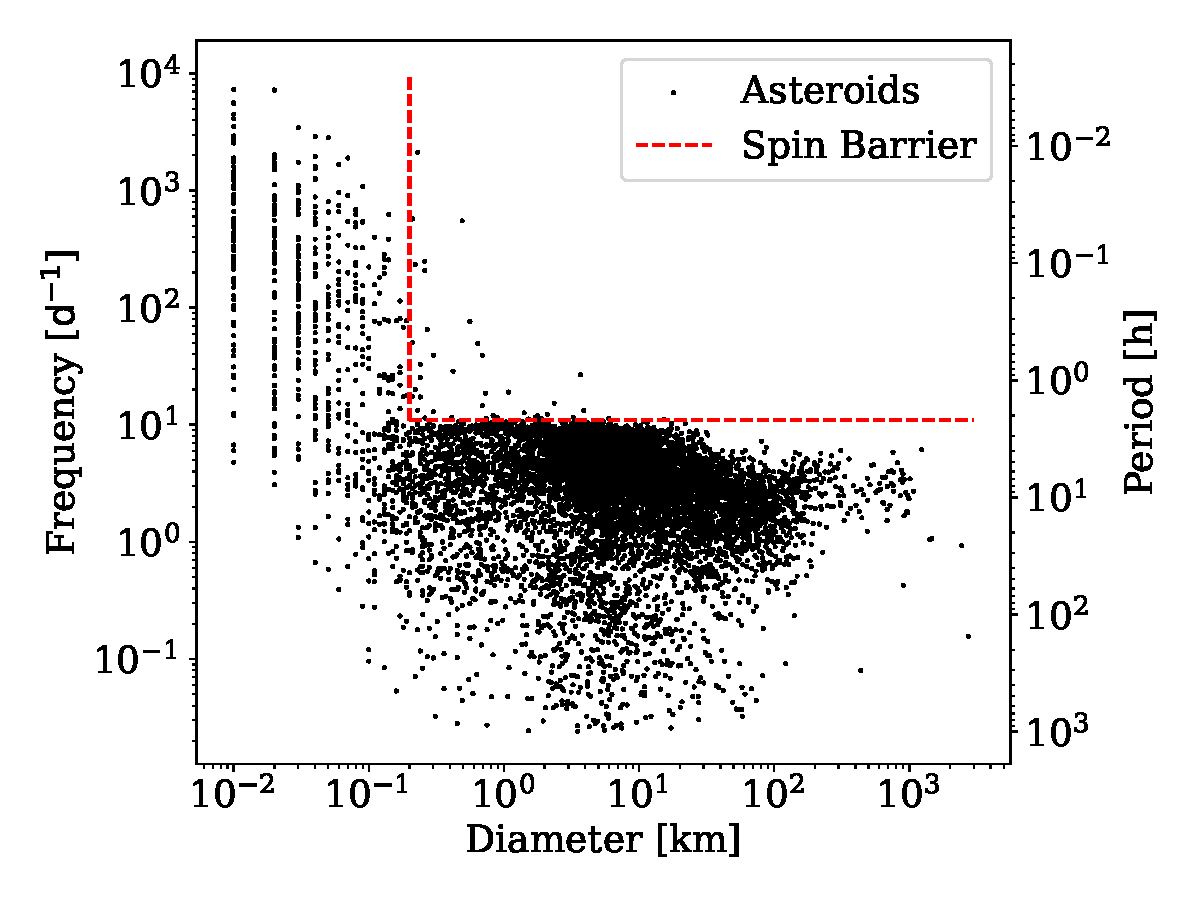
\includegraphics[width=0.7\textwidth]{../Test Code/Testing Figures/Diam-FreqPlot.pdf}
  \caption[Asteroid frequencies vs diameter (LCDB)]{The $U\geq 2-$ rotation frequencies in \unit{\per\day} and the inverse as a period in \unit{\hour} againts the diameter of the body in the October \nth{1}, 2023 LCDB \citet{Warner2009}.
    This is using the diameter of the asteroids from the LCDB $H$ to diameter conversion. The spin barrier of \citet{Pravec2000} is shown in red dashed lines}
  \label{Fig:FreqVsDiam}
\end{figure}

\subsubsection*{Interstellar Objects}
%Omuamu
High amplitude variation has come to the forefront of questions about asteroid properties because of the first interstellar object, 1I/\omuamua \citep[see][for a review]{Bannister2019}.
\omuamua was determined to be spectroscopically red \citep{Fitzsimmons2017, Meech2017}, and having a photometric colour in the neutral end of the solar system range \citep{Bannister2017}.
1I was classed as asteroid due to lack of a coma, and no noticeable activity.
This contrasts the second ISO, 2I/Borisov, which had many cometary characteristics \citep[see ][for a review]{Dorofeeva2023}. %\\TODO cite, as opposed to 2I??
\omuamua was measured to have a rotation period of \qty{8.67(0.34)}{\hour} \citep{Belton2018} and seemed to be tumbling \citep[e.g.][]{Drahus2018,Fraser2018}.
Combing the tumbling with an elongation ratio of up to \qty{6(1)}{}:1 \citep{McNeill2018}, 1I is said to have a cigar shape \citep{Belton2018}.
The peak to peak amplitude variation of this ISO was \qty{2.5}{\mag} \citep{Meech2017} over its double peaked light curve.
This is quite interesting, as it varies more than most asteroids.
With the full sky survey of bright asteroids, we hope to find many asteroids with such a large amplitude variation, and to see just how rare \omuamua is.

\section{Methods}\label{Sec:Meth}

\subsection{Querrying Databases}\label{SubSec:Querry}

\begin{figure}[h!]
  \begin{subfigure}[t]{0.5\textwidth}
    \centering
    \includegraphics[width =\textwidth]{../Test Code/Testing Figures/interpPos\_22\_2\_3\_4.pdf}
    \caption[Positions]{Positions of asteroids in a cut.}
    \label{Fig:interpPos}
  \end{subfigure}
  ~
  \begin{subfigure}[t]{0.5\textwidth}
    \centering
    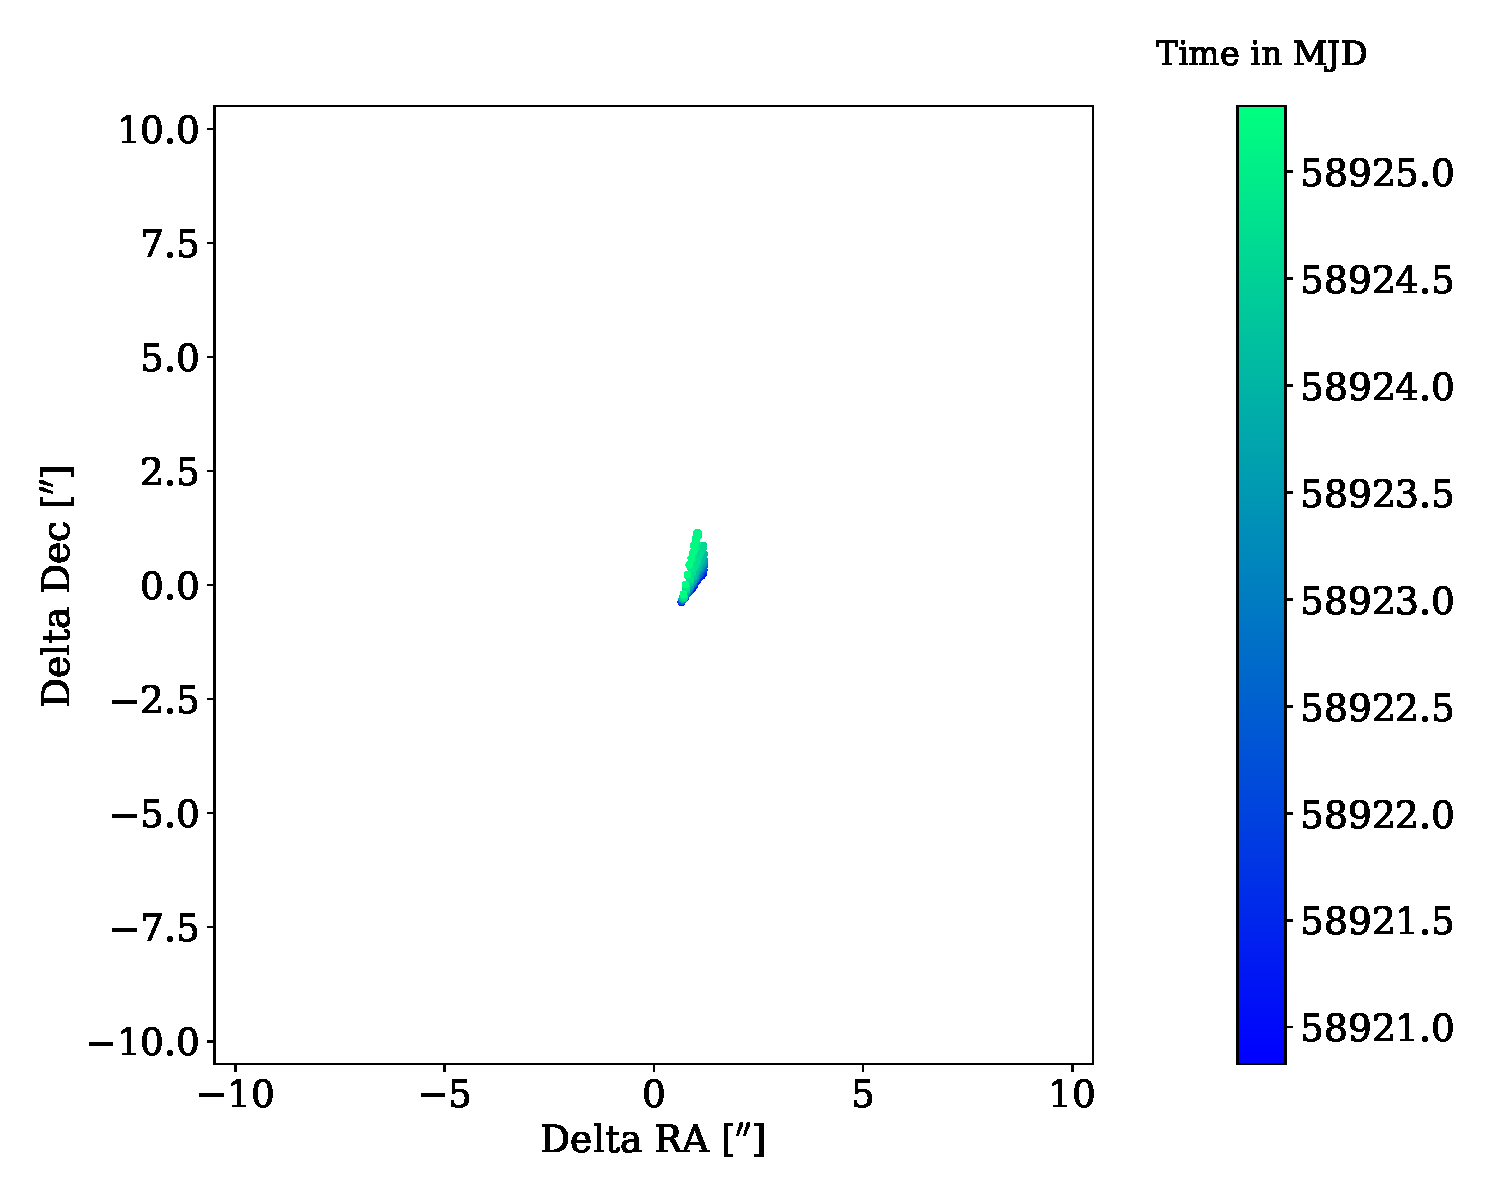
\includegraphics[width =\textwidth]{../Test Code/Testing Figures/1989 BC1PosCheck.pdf} %TODO one with more points???
    \caption[Errors]{Error in interpolated positions}
    \label{Fig:errPos}
  \end{subfigure}

  \caption[Interpolated positions and error of asteroids]{
    (a)
    The interpolated positions of asteroids in one cut of a TESS sector.
    The colours of the lines are time sequenced, as shown in the colour bar.
    The alpha of the colours are scaled by the absolute magnitude $H$ of the asteroid, queried from JPL Horizons.
    Both celestial (RA and Dec) and ecliptic (ecLon and ecLat) coordinates axes are shown.
    The green $+$ is the centre of the cut.
    This cut was chosen because of how many asteroids there were, enough to see the shape of the box, but not so much that the lines are overwhelming to the eye.\\
    (b)
    The difference in the interpolated position of an asteroid from bulk queries to JPL Horizons, with interpolated coordinate being subtracted from the coordinate returned by Horizons. The colour bar is a different colour map to (a) as the range of time is shorter. The extent of the box is one TESS pixel, \qty{21}{\arcsec}. This is of asteroid ``1989 BC1'', but all others checked are similarly accurate (It is very expensive to check them all by brute force queries of Horizons).
  }
  \label{Fig:interpandErrPos}
\end{figure}

To check for asteroids in the TESS data, the positions of the asteroids with time are required.
For most asteroids, their orbital elements are well known, so it is a matter of looking them up and cross-matching with transients in the TESS data.
Python was used to make API calls to
%{Skybot}\footnote{\href{https://vo.imcce.fr/webservices/skybot/}{Skybot: https://vo.imcce.fr/webservices/skybot/}} 
Skybot \citep{Berthier2006} to get positions of asteroids in a cone search box in right ascension (RA) and  declination (Dec) space.
As TESS sectors are \qty{27}{\day} long, querying every \qty{12}{\hour} is manageable.
These positions are still very sparsely spaced in time compared to the TESS data, so an interpolation is needed to bridge the gap.

Knowing where the asteroids are is helpful for finding them in the archival TESS data, but knowing more about the individual asteroids is also useful for population statistics.
The \texttt{astroquery} \citep{Ginsburg2019} package was use to query JPL Horizons% {JPL Horizons}\footnote{\href{https://ssd.jpl.nasa.gov/horizons/}{JPL Horizons: https://ssd.jpl.nasa.gov/horizons/}} 
was used to obtain the orbital elements of each asteroid, $a$, $e$, and $i$, as well as an absolute magnitude $H$, which is a good proxy for size (as discussed above). %TODO ref



\subsection{Interpolation}\label{SubSec:Interp}



With TESS data coming in $\frac12\unit{\hour}$ chunks, 24 interpolated points are needed between each API call.
These interpolated positions can be seen in \autoref{Fig:interpPos} for a cut from \texttt{TESSELLATE}.
There are a few interesting features, such as the asteroids are moving in the same direction, indicated by the colouring, they come in from low RA and Dec and tend to increase both coordinates as the month of the sector progresses.
There is also a large size range in this slice of sky, ranging over \qty{5}{\mag} in absolute magnitude, which can be seen in the alpha (or transparency) of the tracks in \autoref{Fig:interpPos}.
Because of a small change in position between each frame, \citep[$\sim \qty{1}{\px}$ per frame][]{Pal2018}, this interpolation should be accurate.
The
Checking against a higher frequency query to the JPL Horizons ephemeris  confirmed this accuracy on a few asteroids, as shown in \autoref{Fig:errPos}.
This is not a feasible way of getting all the positions, as the queries are per name and time, not per area and time like the cone search in Skybot.
They are also rate limited, so while a few asteroids can be checked, filling the gaps between the Skybot half day queries for all the asteroids would take far too long.
For the faster TESS FFIs, more interpolated points are needed, but a smaller the change in position between each point will be.
Forcing the interpolations to be at the same time as the TESS frames, which are known thanks to \texttt{TESSELLATE} saving them out, simplifies the matching to detections and forced photometry of these points.



\subsection{Detection Matching}\label{SubSec:Match}

%Match to detections
Matching these interpolated positions to \texttt{TESSELLATE} detections is important to lower the unknown transient outputs of this pipeline.
Having interpolated their positions, the asteroids have a well sampled set of RA, Dec and time values of where they should be in the TESS data.
They should show up in a pixel for a small number of frames, of order $\sim1$.
This is the same as a lot of other transient events, a sharp rise in brightness and then disapering quickly again.
The number of frames do change, type Ia supernova will brighten is a matter of a few hours and then dim for days, while stellar flares are of similar profile by a smaller max brightness and a corrsepondingly shorter decay time.
Asteroids are very short spikes, however these detection pipelines are robust. %? Clarinda begs to differ
These pipelines have already found the aforementioned supernova, stellar flares and variable stars, by matching to catalogues of those types of objects (Gaia, ZTF etc.).
The job of this work is to catch all the asteroids in the set of all the transients that are returned from the pipeline.
To do this, catelogue matching is in order.


Using the \texttt{KDTree} algorithm \citep{Maneewongvatana1999} as implemented in \texttt{SciPy} \citep{2020SciPy-NMeth}, the RA and Dec coordinates of the interpolated points and the detections can be compared and matched together.
Filtering this \texttt{KDTree} output by restricting the time between spatially coincident matches to less than \qty{0.1}{\day} stops any accidental matches in position from non-asteroid detections.
A cut is then made by smallest distance, in coordinate space, and any distance must be smaller than \qty{0.01}{\degree} (\qty{36}{\arcsec}), which is within 2 TESS pixels.
Then, if multiple detection match to the same interpolated point, the detection with the smallest distance will be taken.
An example of the matches found using this \texttt{KDTree} is shown in \autoref{Fig:RADecMatch}.
It is clear that \texttt{TESSELLATE} is not detecting every frame that an asteroid is in.
Detctions in \texttt{TESSELLATE} are done on a per pixel basis, and asteroids only cross each pixel for a short number of frames.
Not every interpolated point gets a match, due to a variety of reasons, which culminate in there being not an extreme enough of a difference between frames at that pixel location.
Instead there are bunches of freqntly matched points, and then patches where there are few matches detected at all.

%TODO fig for agregate of all asteroids in a sector, to go in results 

\begin{figure}[]
  \centering
  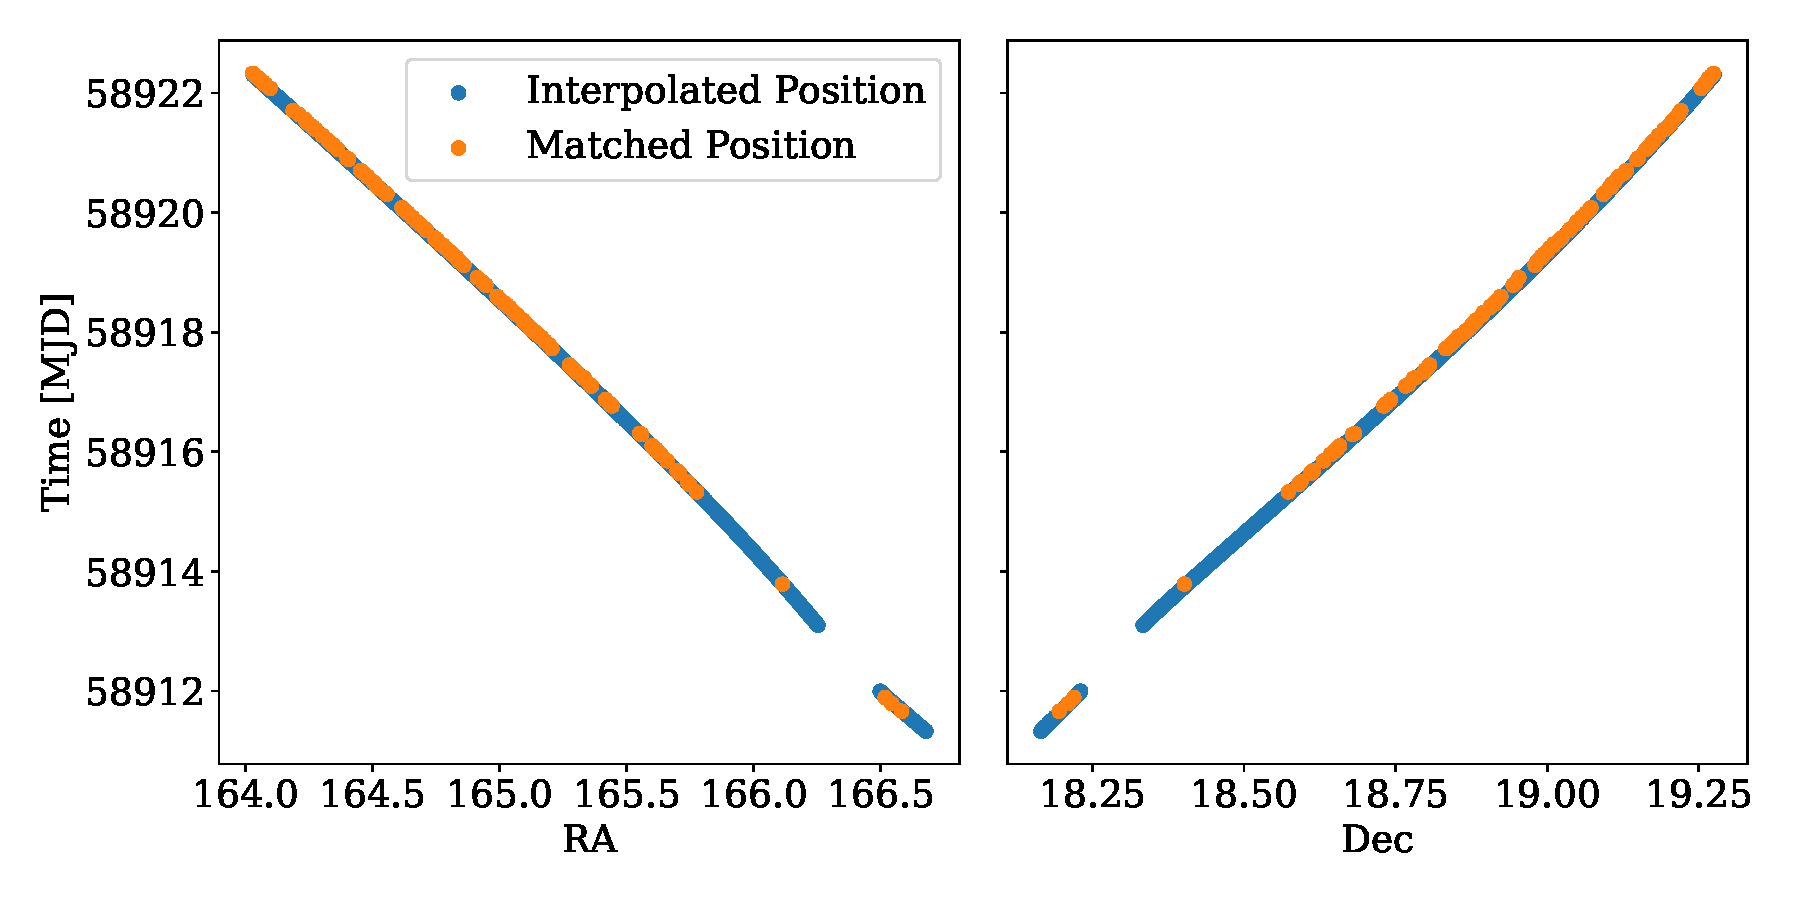
\includegraphics[width =\textwidth]{../Test Code/Testing Figures/DetectMatchPos.pdf}
  \caption[Interpolated and Detected Positions]{The RA (right plot) and Dec (left plot) of the interpolated points (blue) and the matched \texttt{TESSELLATE} sources(orange) against the time. The gap is from the TESS downtime in the sector, when it was passing close to earth.}
  \label{Fig:RADecMatch}
\end{figure}

\subsection{Ligthcurves}\label{SubSec:Lightcurves}

%light curves; detected VS forced interpolated 
There are two sets of points to take light curves from.
The matches from the detections, which already have a flux calculated, and the interpolated points themselves, which are more numerous but require forcing the photometry.
There were some challenges getting the flux of the interpolated points, even when \texttt{TESSELLATE} has already reduced all the FFIs of interest.

Using the \texttt{SkyCoord} module of \texttt{Astropy}, the world coordinates, in RA and Dec, can be transformed into pixel coordinates, $x$ and $y$, using a world coordinates system (WCS) from TESSELLATE.
\texttt{Photutils} \citep{Bradley2024} was then used to do aperture photometry with a \qty{1.5}{\px} radius to account for the spread in the TESS PRF. %?cite PRF

The integer coordinates of the asteroids seemed to be leading the object in any given frame of TESS. %?FIG?
This was decreasing the total flux of the asteroid, as the box used for sumation of the fluxes was hitting mostly sky.
This also caused a ``sawtoothing'' effect, where the lighturve would jump from a minimum to a maximum when the integer coordinate snaped from being a pixel out to back on the asteroid.
This both of these issues can be fixed by calculation of the centre of mass (COM) flux, the average brightness in $xy$ space on a $5\times5$ cut of the image centred on the interpolated position.
I didn't take the highest pixel value in this box because there could be a rouge star in the field that it snaps to, instead of the asteroid.
A \texttt{Photutils} aperture photometry call to this COM with a radius of \qty{1.5}{\px} was enough to get fluxes of the same order, but with a far more smooth transition from maximum to minimum, as expected from rotating asteroids.

%TODO data cleaning explaination
Following \citet{McNeill2023}, any fluxes more than $3\sigma$ from the mean value are sigma-clipped from the forced photometry lightcurves.
This does introduce gaps into an otherwise regularly sampled lightcurve, but the contamination from background stars the object is passing in front of is too great.

\begin{figure}
  \centering
  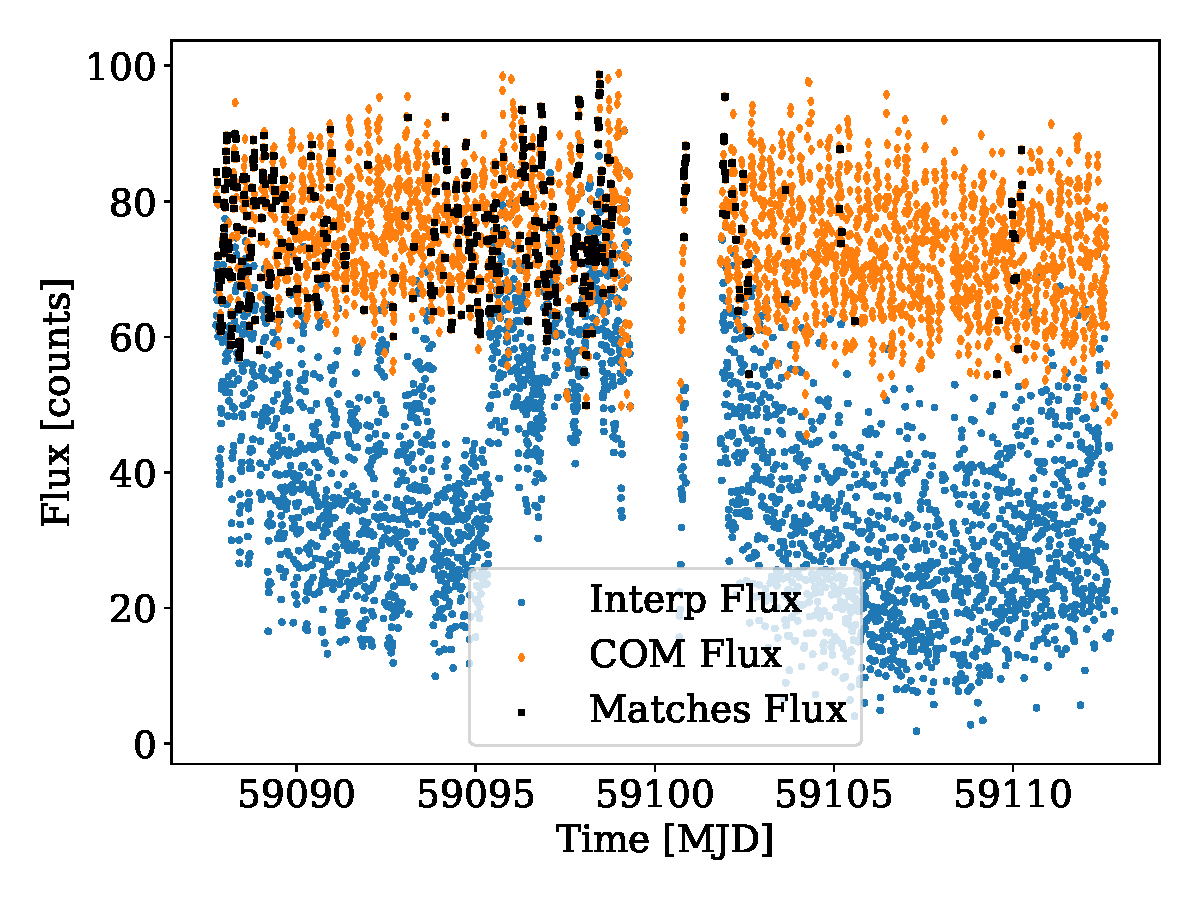
\includegraphics[width =\textwidth]{../OzData/SingleBodyLC1991 VT.pdf}
  \caption[Light curves of 1991 VT]{The light curves of the asteroid 1991 VT throughout its entrie journey across sector 29, with the flux of the interpolated positions in blue circles and the flux from the COM in orange diamonds, and the \texttt{TESSELLATE} flux for any matched points in the black squares.
    The Flux axis is measured in counts, as calculated by \texttt{TESSreduce}, and the times are in modified Julian date (MJD).}
  \label{Fig:FullSingleLC}
\end{figure}
A comparison between the three light curves is interesting, as one might expect only the brightest parts of the lightcurve will be matched.
\autoref{Fig:FullSingleLC} shows these three light curves for a single body.
The COM flux seems much more stable than the interperted flux on its own, and at a higher average flux count.
This should result in more accurate periodograms as there is less overall curve to the data.
The matched points are comparatavely sparce for this object, which is not the case for all.
Many have no matches, and some have almost fully matched, this will be discussed more later.







\subsection{Period detection}\label{SubSec:Periods}

%Periods and amplitueds for everything detected

The next part of my analysis has to do with determining the periods and amplitudes of each asteroid's light curve.

A widely used technique in determining the periods of astronomical data is the Lomb-Scargle periodogram \citep[\citet{Lomb1976,Scargle1982}, but see][for a review]{VanderPlas2018}.
This method can efficiently take discrete timeseries data of which the observations are unevenly spaced and calculate the frequencies present in the sample.
TESS should have rather evenly spaced data, as the FFIs are produced on a set cadence, but sometimes data will be missing.
For example, it may have been sigma clipped due to a spike in brightness that is unphysical for an asteroid, or TESS sees the same asteroid in the same sector on either side of the day long mid-sector break it takes for data transfer.
The Lomb-Scargle periodogram deals with this uneven sampling much better than either a fast Fourier transform or a direct least squares fit.

There are a few different implementations of a Lomb-Scargle periodogram available in world of astronomy python packages.
I first tried using the \texttt{Lightkurve} \citep{Lightkurve2018} package built for period analysis of TESS (and Kepler) data of variable stars.
\texttt{Lightkurve} was easy to use but didn't allow for fine-tuning of the periodogram, or give any model of the curve it produced.
The next option was peeling back a layer of abstraction and using the Lomb-Scargle periodogram as implemented by \texttt{Astropy}\citep[\citet{Astropy2022} but see][for the implementation]{Vanderplas2012,Vanderplas2015}.
There were interesting similarities and differences between the packages.
\texttt{Lightkurve} is based on the \texttt{Astropy} methods, but does not give all the functionality, instead opting to simplify the process.
\texttt{Astropy} gives a statistic on how confident it is in the detected frequency is, the false alarm probability.
It also returns a model, in the form of

\begin{equation}
  \label{Eq:LCModel}
  F(t;f,\vec{\theta}\,) = \theta_0 + \theta_1\cdot\sin{2\pi ft} +\theta_2\cdot\cos{2\pi ft}
\end{equation}

where the flux, $F$, is given in terms of time, $t$, the calculated frequency, f, and the model parameter $\vec{\theta} = [\theta_0, \theta_1,\theta_2]$.
These parameters are useful in reconstructing the sinusoid without rerunning the periodogram.
The method used for the periodogram fits is the new \texttt{nifty-ls} package \citep{Garrison2024} that has can be implemented on its own, or by interfacing with \texttt{Astropy}.
I use the later implementation as the speed up from the nonuniform fast Fourier transform is helpful on the large dataset from \texttt{TESSELLATE}, but the astropy interface is how I had everything set up to run on just one cut.

I an using a frequency window of for the periodogram between the the inverse of twice the time the asteroid spends in the sector and the Nyquist frequency (1/TESS cadance).

%???
There will be differences in the period between the matched points and the interpolated points, not just because of the difference in average flux, but also from the larger number of points. This difference needs to be carefully thought through to understand what is the more likely period.

%TODO single object periodogram
%Maybe a bad one too

\subsection{Asteroid Statistics}\label{SubSec:StatMeth}

%Run on server
The \texttt{TESSELLATE} pipeline has been running on the OzSTAR supercomputing facilities.
After I was confident that all the parts of the asteroid detection and subsequent light curve analysis worked as required on one cut of one camera of one ccd of one TESS sector, the same code was be refactored slightly to work on OzSTAR and a large-scale analysis of all the processed TESS sectors can be run.

I will be looking for completeness of detections of asteroids, as well as accuracy of periods and amplitude variation by comparison to the LCDB.

The completeness of the asteroid population in TESS as a function of their apparent magnitude can be determined.
The apparent magnitude is one of the properties returned from the queries, and is in the V band.
By taking a limit on the if an asteroid is detected \dots %TODO what is the limit
Breaking the average V mag of these objects into \qty{0.5}{\mag} bins for both the sample returned from a query and the sample detected, a ratio of completeness can be calculated per bin.
(Note: If there are no asteroids in a bin, none have a chance of being recovered, so the all did get recovered. I.e. $\frac{0}{0}=1$, this is only an issue at the brightest magnitude where the fewest asteroids exist.)

\section{Results}\label{Sec:Res}

This is the results for TESS sector 29.
This sector was chosen because it is early in the \qty{10}{\min} cadence of TESS FFIs, and had been fully run through TESSELLATE.
Similar results can be found in any of the sectors, just the computaion time was a limiting factor.

\subsection{Asteroid Properties}\label{SubSec:AstPropRes}

The orbital element properties of the asteroids were returned by JPL Horizons queries.
A plot of the semi-major axis against the other orbital elements, eccentricity and inclination, is shown in \autoref{Fig:AEI}.
The disticntion between the resonances in the main belt are clearly seen. There are lines seperating the middle belt from the inner and outer belt.
The Jupiter trojans are well defined, at just past \qty{5}{\au}, with a small range of eccentricity but a large spread in the inclination.
Inbetween the outerbelt and the Jupiter trojans, sit some Mars crossers.
A some near earth objects (NEOs) at smaller $a$ and a few more objects that are scattered with high $e$ and or $i$ complete the distrabution.

\begin{figure}
  \centering
  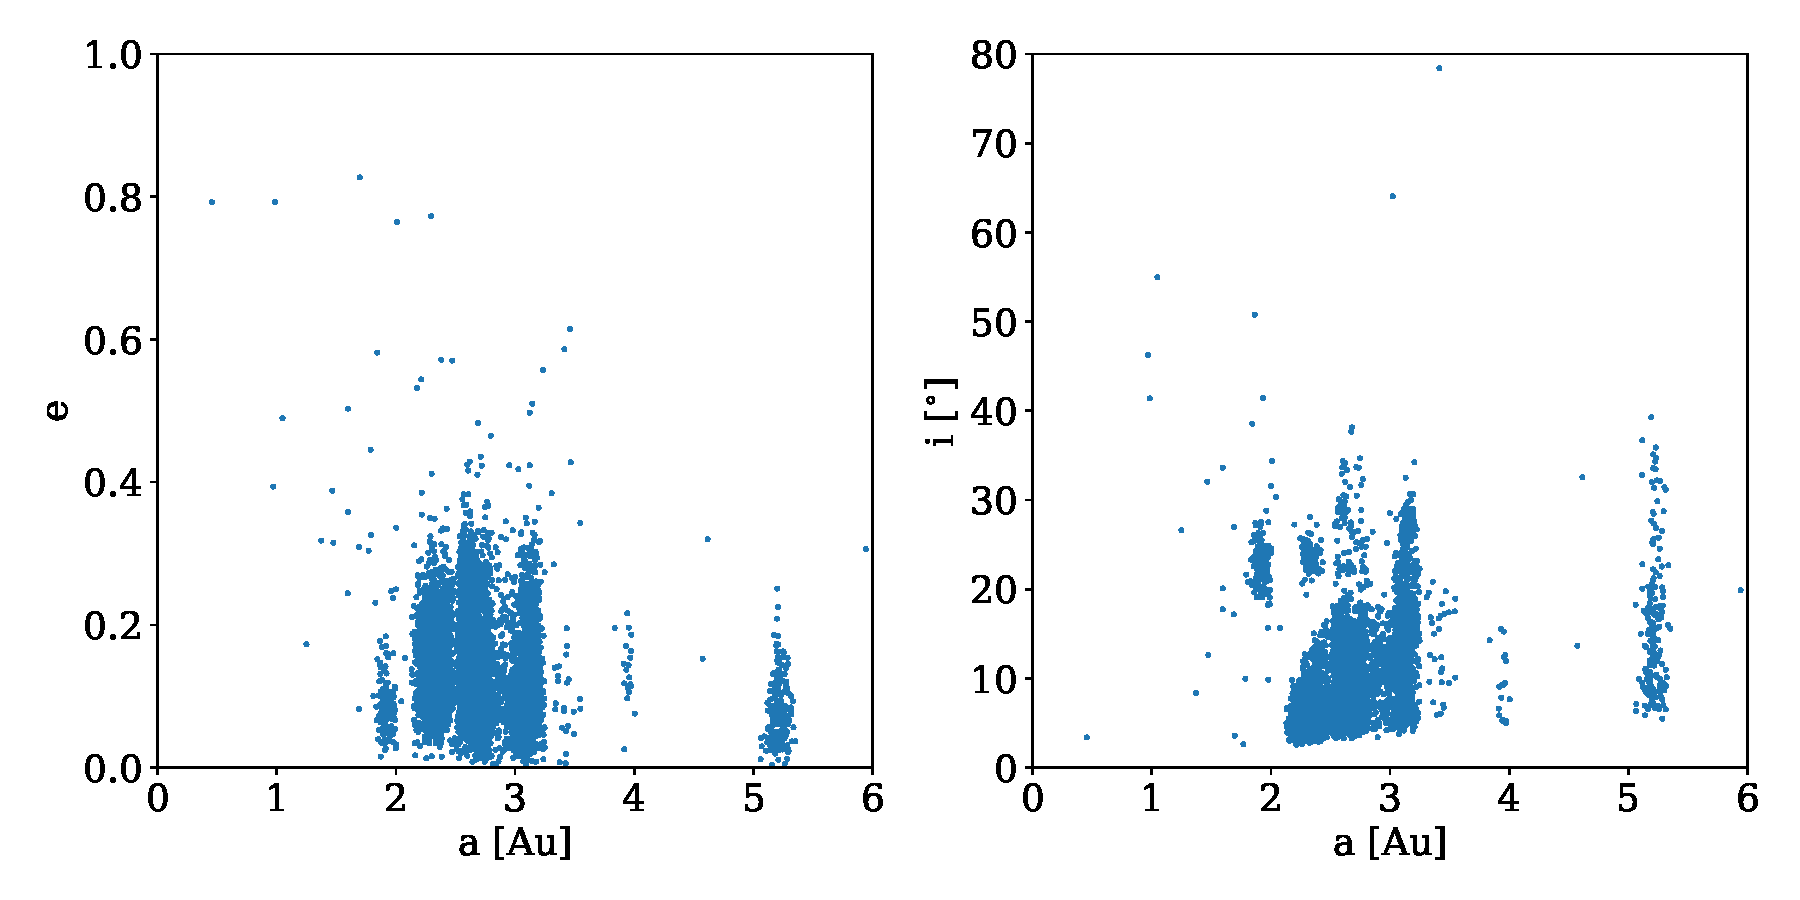
\includegraphics[width=\textwidth]{../OzData/AEIplot29.pdf}
  \caption[aei distribution]{a, e, i, plot of all the objects on sector 29}
  \label{Fig:AEI}
\end{figure}


The number the belong to each class of objects is highlighted in \autoref{Fig:NumPerClass}

\begin{figure}
  \centering
  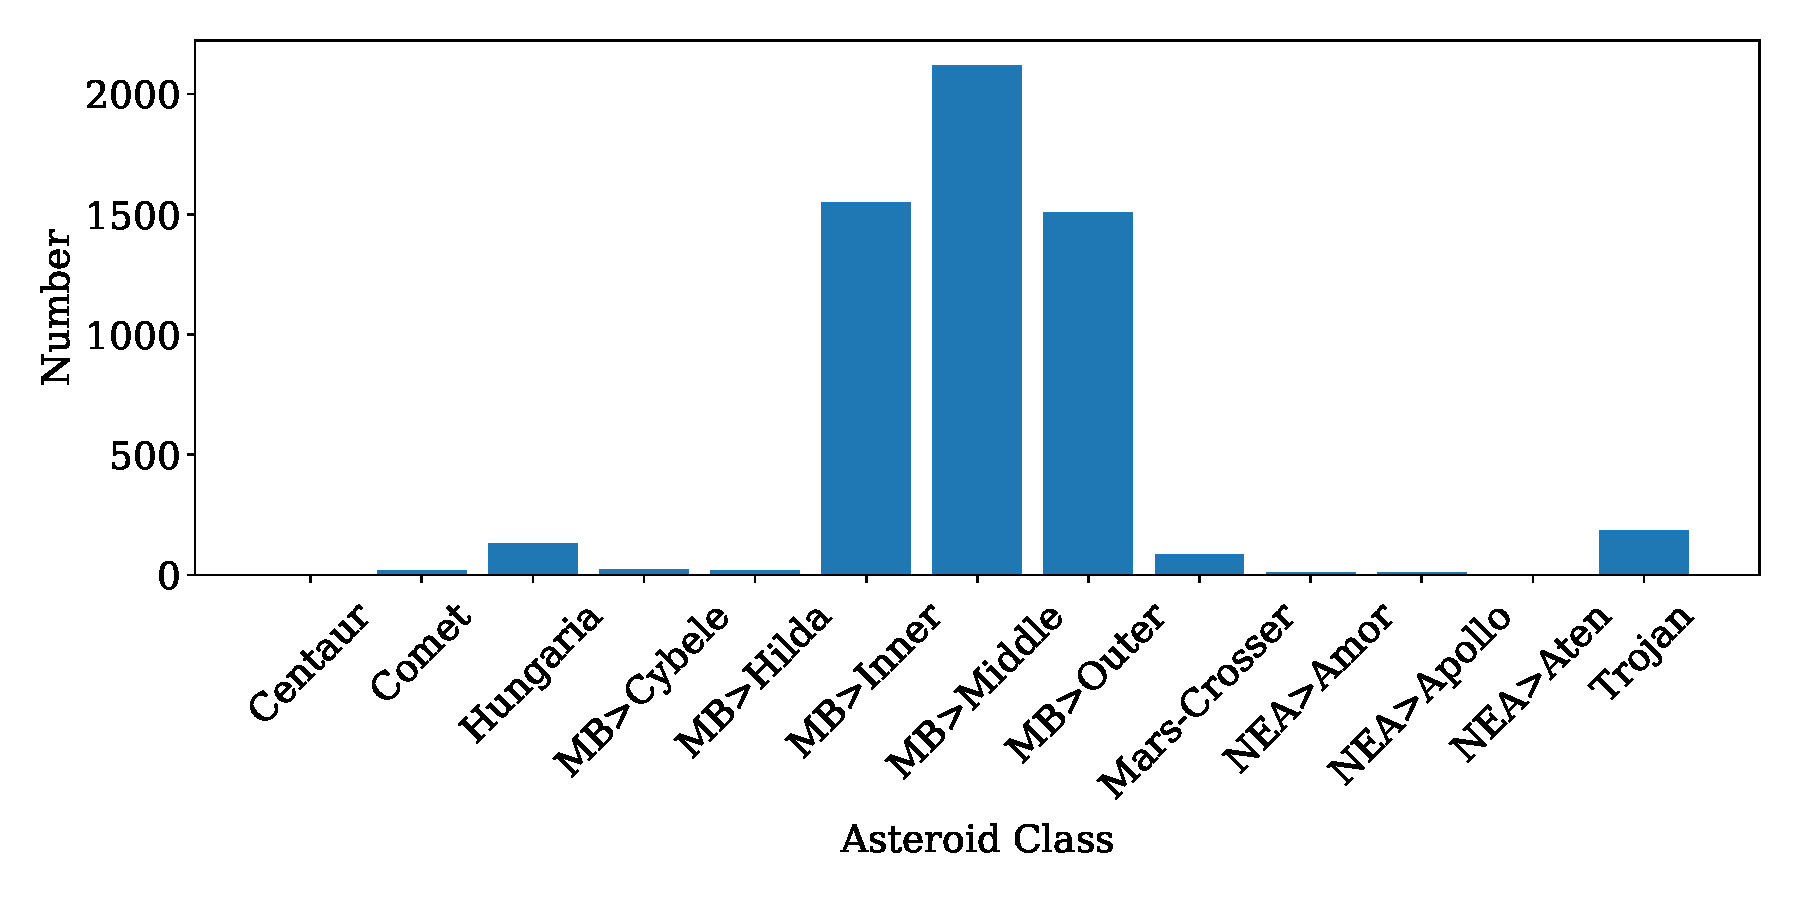
\includegraphics[width=\textwidth]{../OzData/classesBar29.pdf}
  \caption[Class distribution]{A distrabution of the number of asteroids per class that \texttt{SkyBot} knows the object is. }
  \label{Fig:NumPerClass}
\end{figure}

\subsection{Detectability}

\begin{figure}
  \centering
  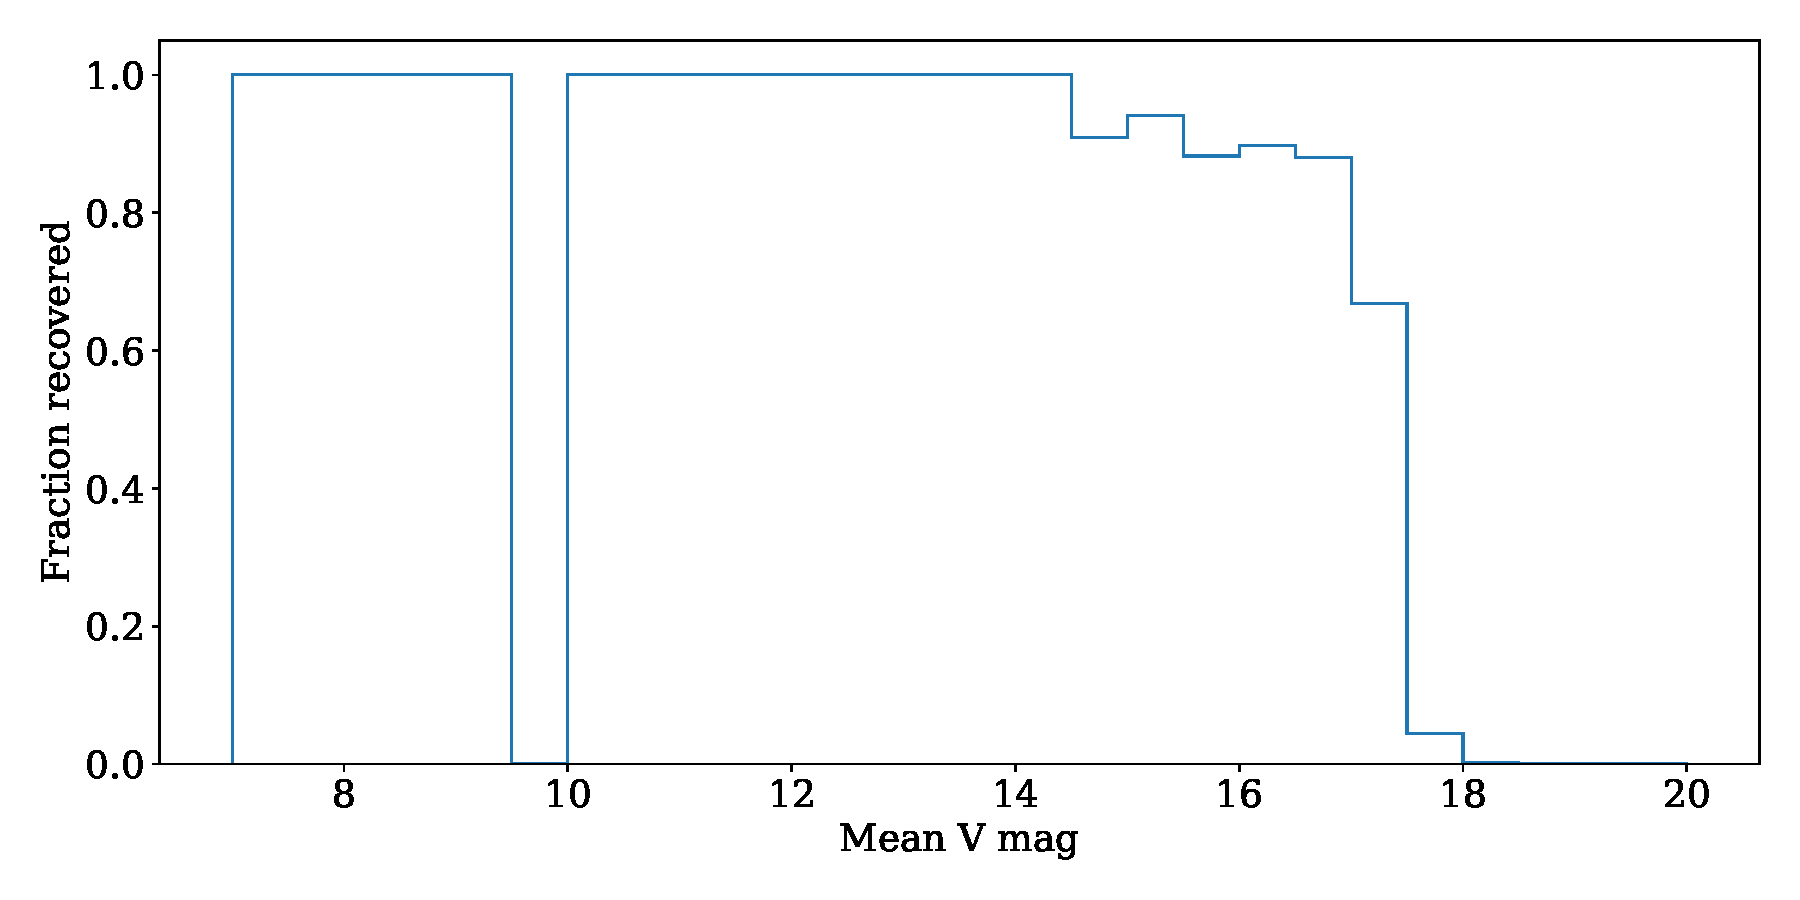
\includegraphics[width=\textwidth]{../OzData/recoverdHistBkgLimof10.pdf}
  \caption[Recovery plot]{A histogram of known average visual magnitude of each object against the whether or not the object has a lightcurve with an average flux value above 10 %!CHECK
    counts for its COM flux.
  }
  \label{Fig:RecovOverBkg}
\end{figure}

\begin{figure}
  \centering
  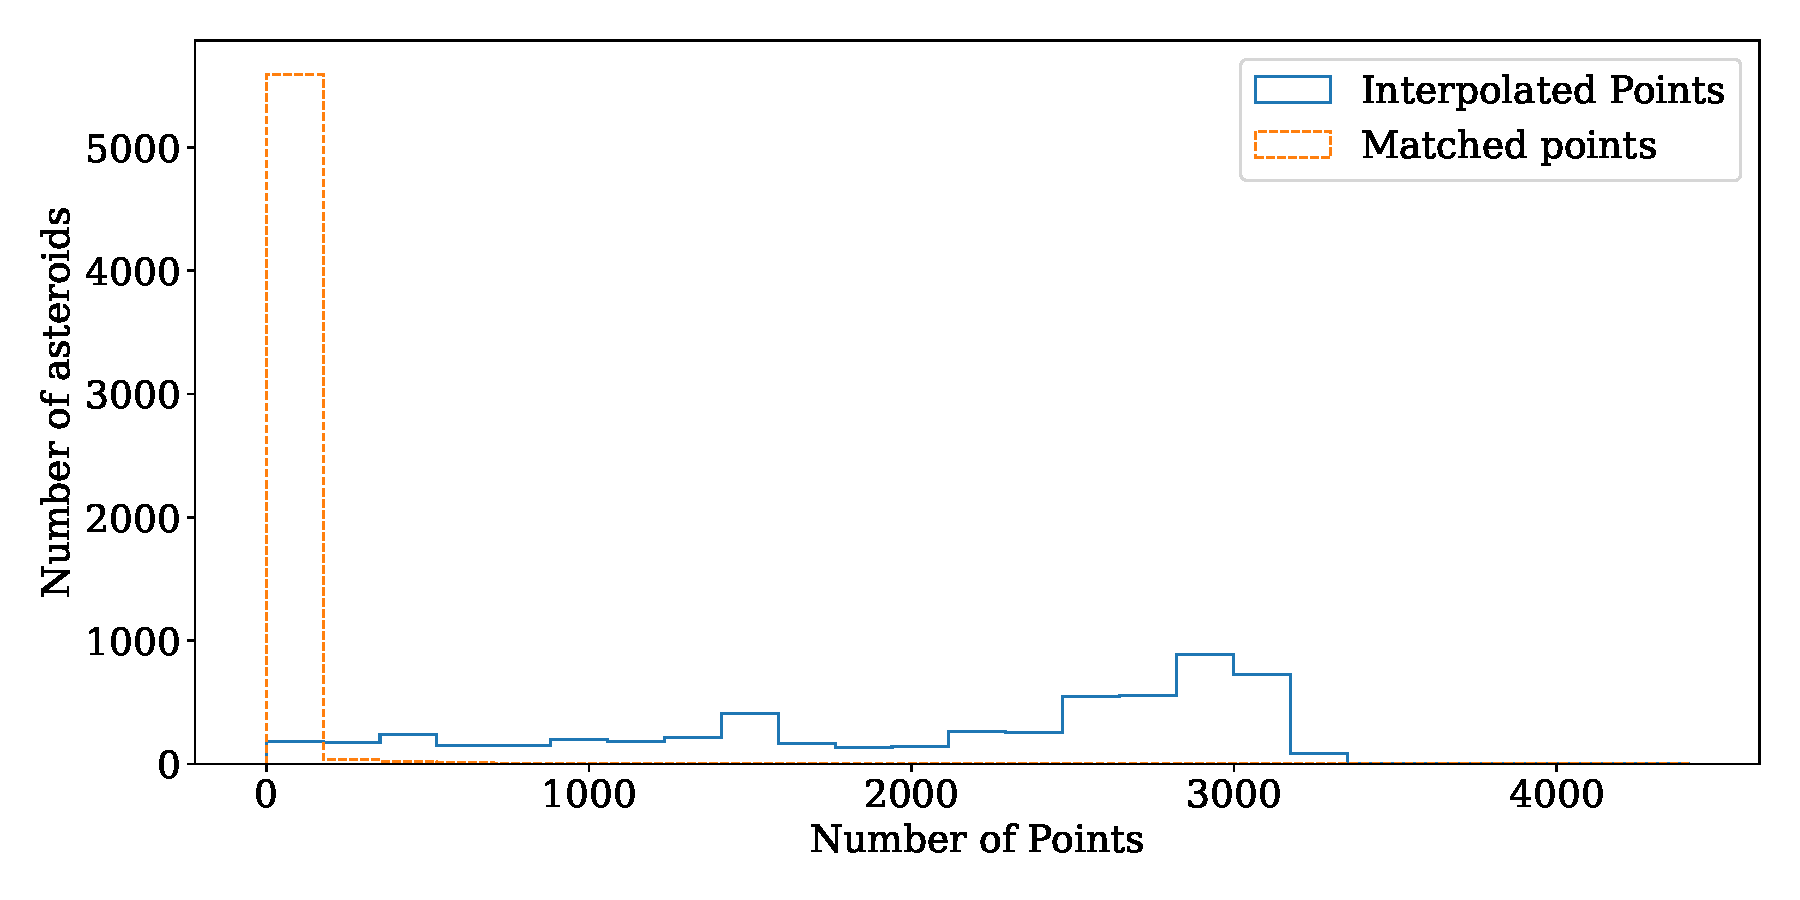
\includegraphics[width=\textwidth]{../OzData/pointsMatchesNumberHistTEST.pdf}
  \caption[short]{A histogram of the number of point in the lightcurve of each asteroid (blue) against the number of matches each asteroid gets in the \texttt{TESSELLATE} detections(orange dashed). }
  \label{Fig:MatchInterpHists}
\end{figure}


\begin{figure}
  \centering
  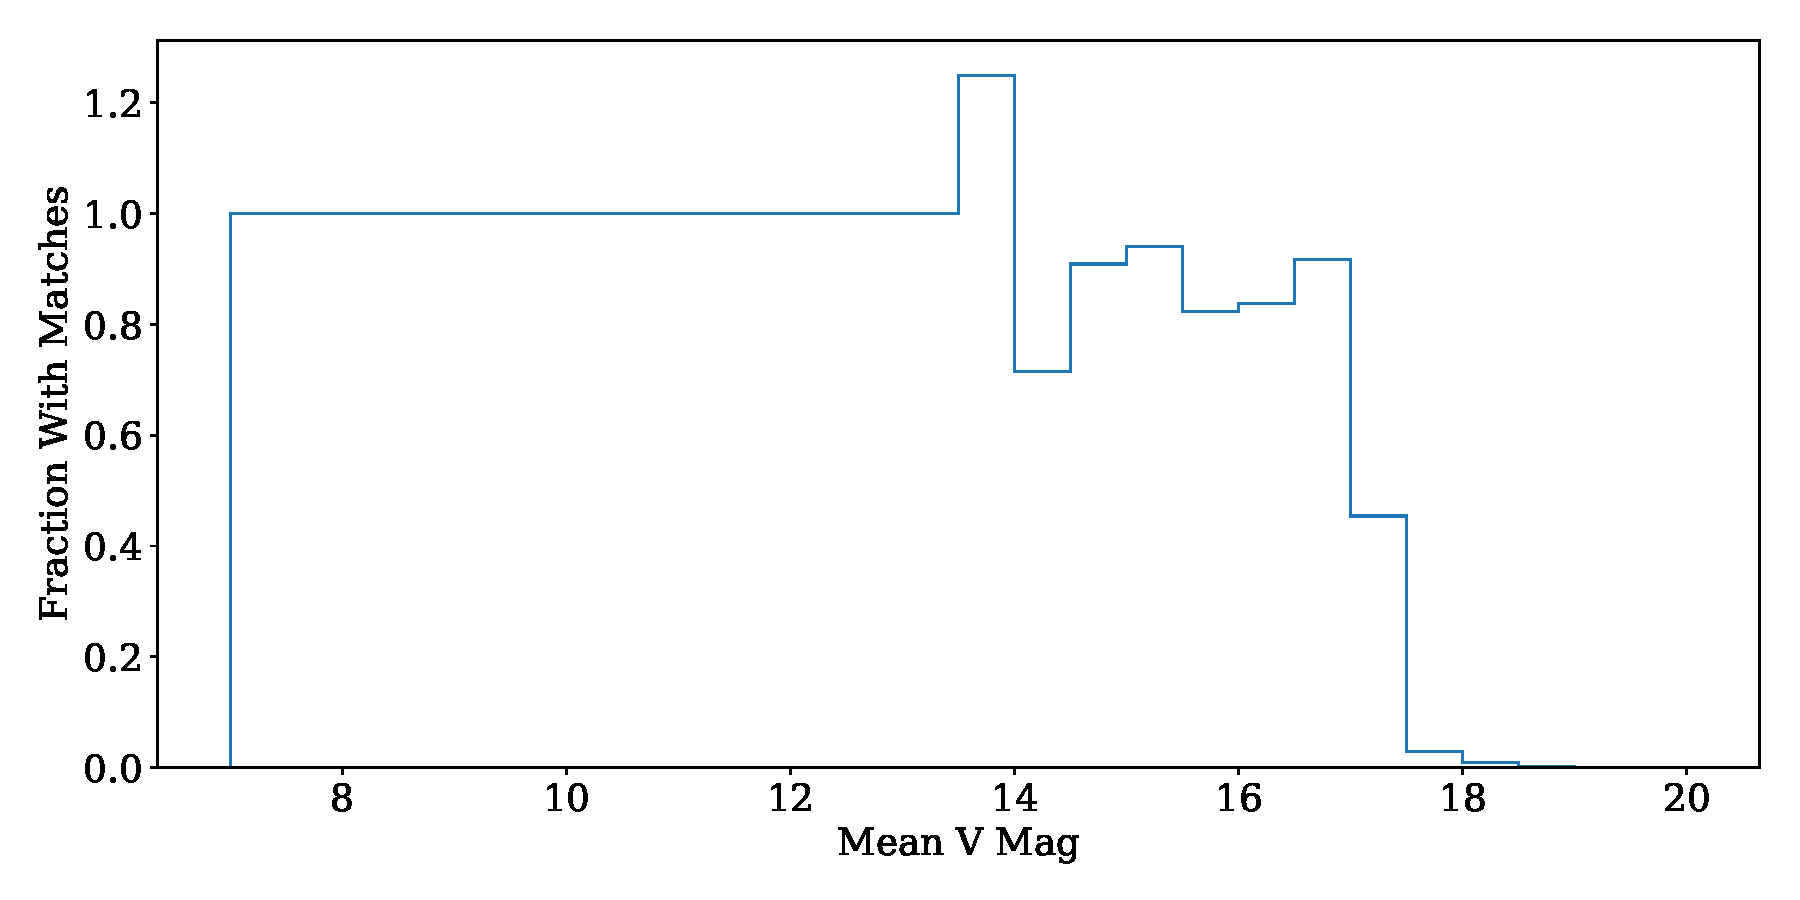
\includegraphics[width = \textwidth]{../OzData/matchesHist29.pdf}
  \caption[Magnitude of matches]{The visual magnitude of the asteroid against the fraction of asteroids in this bin with more than 3 %!CHECK
    matches.
  }
  \label{Fig:MagofMatches}
\end{figure}


\section{Discussion}\label{Sec:Disc}
\section{Conclusion}\label{Sec:Conc}



\newpage %* Page number above here must be <=25

\section*{Acknowledgements}
\addcontentsline{toc}{section}{Acknowledgements}
%OzSTAR asks for:
\small
This work was performed on the OzSTAR national facility at Swinburne University of Technology.
The OzSTAR program receives funding in part from the Astronomy National Collaborative Research Infrastructure Strategy (NCRIS) allocation provided by the Australian Government, and from the Victorian Higher Education State Investment Fund (VHESIF) provided by the Victorian Government.

This research has made use of data and/or services provided by the International Astronomical Union's Minor Planet Center.

This work has used data and/or services provided by NASA's Solar System Dynamics website, \url{https://ssd.jpl.nasa.gov/}. Specifically JPL Horizons: \url{https://ssd.jpl.nasa.gov/horizons/}.

This research made use of Photutils, an Astropy package for detection and photometry of astronomical sources \citep{Bradley2024}.

%*Bib
\addcontentsline{toc}{section}{References}
% \bibliographystyle{jphysicsB}
\bibliography{bibfile.bib}
\end{document}



